\chapter{Efficacy of Transformation}

\section{Comparison of methods}
\null \quad \quad In Chapter $5$ we determined the complexity of computing a query over a DAG $G$, the complexity of finding an edge reversal in $G$ such that $\Delta(G,q)$ is reduced via the \textit{greedy strategy}, and of recalculating the probabilities of graph after edge reversal. The result is a fully specified DAG $G'$ which is Markov equivalent to $G$ such that answering $q$ on $G'$ is faster than answering $q$ on $G$. However, we must now compare the speedups earned in answering $q$ on $G'$ instead of $G$ with the cost of transforming $G$ into $G'$. We will also consider these results in the context of sequences of queries, rather than individual queries. \newline
\null \quad \quad In this chapter, we continue enforce restrictions on the DAG $G$ outlined in~\cref{section:complexityofaquery}: that the maximum number of cycles in $G$ is in $\mathcal{O}(log(|V|))$, that the maximum degree of a vertex is in $\mathcal{O}(log(G))$, that $G$ is sparse, and that $G$ has binary variables. \newline
\begin{table}[h!]
  \begin{center}
    \begin{tabular}{ l  l }
	\quad The cost of answering a query $q$ on $G=(V,E)$ 		& $\mathcal{O}(2^{|V|})$ \\[1em]
	\quad The speedups earned by reversing $n$ edges in $G$		& $\mathcal{O}(2^{n})$ \\[1em]
	\hline \\
	\quad  The cost of finding all covered edges 				& $\mathcal{O}(|V| \cdot log(|V|))$ \\[1em]
	$+$ The cost of finding $\Delta(G',q)$ for all covered edges 	& $\mathcal{O}(|V|^{5})$\\[1em]
	$=$ The cost of finding an advantageous edge reversal 		& $\mathcal{O}(|V|^{5})$ \\[1em]
	\hline \\
	\quad The cost of calculating an edge reversal					& $\mathcal{O}(|V|)$ 
    \end{tabular}
      \caption{}
      \label{tab:complexitytable}
  \end{center}
  \end{table}
\null \quad \quad The calculations in Chapter $5$ revealed the complexities shown in Table \ref{tab:complexitytable}.
While calculating the edge reversal itself is less costly than answering a query, we immediately see that the most expensive component of the \textit{greedy strategy} is determining the optimal reversal to make. \newline
\null \quad \quad We also notice that finding the entire set of covered edges in $G$ only has to be done once, since reversing an edge only changes the set of covered edges locally. That is, only edges adjacent to the reversed edge can switch whether they are covered after the reversal. By the assumption that vertices in the graphs have a small number of parents (specifically $\mathcal{O}(log(|V|)))$, this is fast to check. After the set of covered edges is found, multiple reversible edges can be evaluated and reversed without calling \textsc{Find\_Covered\_Edges} again. Therefore, the overhead cost of $\mathcal{O}(|V|)$ only applies once for finding transformations of a given graph $G$. \newline

\begin{theorem}\label{thm:reversalbenefit}
Identifying and reversing beneficial edges is always worth the computational improvement earned from reversal for graphs with $|V|$ \textgreater \ $22$. That is, the complexity of identifying and reversing a beneficial edge is at most as much computational cost as the query saves.
\end{theorem}

\begin{proof}
The complexity of finding covered edges and reversing a beneficial one is $\mathcal{O}(|V|^{5})$. The computation of a query is halved whenever $|\Delta(G,q)|$ is reduced by $1$. Therefore, by finding approximate integer solutions to $2^{|V|} = |V|^{5}$, we see that $2^{|V|}$ is larger whenever $|V| \not\in [2,22]$.
\end{proof}

\begin{remark}
Note that Theorem~\ref{thm:reversalbenefit} does not imply that reversal is \textit{not} worth doing whenever $|V|$ \textless \  $22$, but rather, that it isn't necessarily, but still may be.
\end{remark}

\begin{remark}
While $2^{|V|}$ is a fixed quantity because it corresponds to a fixed number of possible events described by the distribution, $|V|^{5}$ is a worst-case complexity which could likely be reduced with more effective algorithm design. The bound of $V$ \textless \ $22$ is certainly not strict in practice, and it is likely possible that edge reversal could become advantageous for smaller graphs as well. One can reasonably adopt the heuristic that edge reversal is generally advantageous. A promising area for future research is to develop more effective algorithms to reduce the cost of finding beneficial edges to reverse. 
\end{remark}

\section{Reversal in the Context of Multiple Queries} 
\null \quad \quad In this section, we explore the benefits and limitations of edge reversal if we consider a sequence of queries $Q = \{q_{1}, q_{2}, ..., q_{n}\}$ instead of a single query $q$. For example, if we have observable medical data about patients and we wish to determine whether they have multiple diseases (but not the likelihood of them having several diseases simultaneously), we may wish to answer multiple queries consecutively. \newline
\null \quad \quad Answering a sequence of queries $\{p(X_{1}), p(X_{2}), ..., p(X_{n})\}$ is different than answering a single query with multiple targets, $p(X_{1}, X_{2}, ... X_{n})$ in several ways: the former quantifies each probability as individual events, whereas the latter considers the likelihood that both diseases are present simultaneously. Additionally, a sequence of queries allows us to look at different conditions for each query. For example, if $p(X_{1})$ is relevant to the condition $Y_{1}$ in a DAG $G$, but $X_{2}$ is not, then we can simply answer the queries separately ($p(X_{1}|Y_{1})$ and $p(X_{2}$)), rather than considering every condition in both queries. \newline
\null \quad \quad While answering a sequence of queries $Q=\{q_{1}, q_{2}, ..., q_{n}\}$ allows us to determine the probabilities of multiple variables individually, it is also an expensive process since each query must be computed independently. However, knowing the sequence of queries in advance gives us the advantage of being able to consider which graph transformations may be beneficial to the entire sequence, and further, how we might permute the sequence before transforming to reduce the costs of querying. 

\subsection{Universal Effects}

\begin{theorem}\label{thm:universalrev}
Given a DAG $G$ and a reversible edge $(X,Y) \in E$, there is no universally beneficial edge reversal. That is, we can always find a query $q$ such that computing $q$ is more costly after reversing $(X,Y)$ to $(Y,X)$. 
\end{theorem}

\begin{proof}
To demonstrate this, we show that we can always find a query $q$ such that $|\Delta(G,q)|$ is increased when $(X,Y)$ is reversed to $(Y,X)$. Let $G$ be a DAG, and let $(X,Y)$ be an arbitrary edge in $G$. Then $X \in \alpha(Y)$. Let $q = p(X)$. A query of this form depends on exactly $X \cup \alpha(X)$, since it has no conditions and is in the general case by default. \newline
\null \quad \quad Suppose $G'$ is the graph achieved by reversing $(X,Y)$ to $(Y,X)$ in $G$. Then, $Y$ is added to $\alpha(X)$ in $G'$. $X$ still depends on all other vertices in $\alpha(X)$ since we have only added a parent, not removed any. Therefore, $\Delta(G,q)$ now includes the vertex $X$, meaning that $|\Delta(G,q)|$ has grown by $1$. Recall that by Lemma~\ref{lemma:onevertex}, since $(X,Y)$ is a covered edge, $X$ and $Y$ share a set of parents, so the query's cost is only increased by $1$. Thus, since the result that $|\Delta(G',q)|$ \textgreater \ $|\Delta(G,q))|$ is independent of all other properties of $G$, and the chosen edge is arbitrary, we conclude that we can always find such a query $q$. 
\end{proof}

\begin{remark}
A rephrasing of~\ref{thm:universalrev} is that for a set of queries $Q = \{q_{1}, q_{2}, ..., q_{n}\}$, there is not necessarily a single edge reversal which benefits the entire set simultaneously. 
\end{remark}

\begin{definition}
Let $G$ be a DAG, and let $q_{1}$ and $q_{2}$ be queries. If an edge reversal of $(X,Y)$ in $G$ is detrimental to $q_{1}$ but beneficial to $q_{2}$, we call $q_{1}$ and $q_{2}$ \textbf{conflicting queries}. If the reversal is beneficial to both or detrimental to both, we call them \textbf{coinciding queries}. If $|\Delta(G,q_{1})|$ is unaffected by an edge reversal, we call $q_{1}$ a neutral query with respect to the edge. 
\end{definition}

\begin{center}
\begin{figure}[h!]
\centering
\begin{tikzpicture}
\Vertex[x=-4.5, size=.5, color=white, label=$X$]{x1}
\Vertex[x = -2.5, size=.5, color=white, label=$Y$]{x2}
\Vertex[y = 1.5, x=-3.5 ,size=.5,color=white, label=$Z$]{x3}
\Edge[Direct, distance=0.5](x3)(x1)
\Edge[Direct, distance=0.5](x3)(x2)
\Edge[Direct, distance=0.5](x1)(x2)

\Vertex[size=.5, color=white, label=$X$]{x1}
\Vertex[x = 2, size=.5, color=white, label=$Y$]{x2}
\Vertex[y = 1.5, x=1 ,size=.5,color=white, label=$Z$]{x3}
\Edge[Direct, distance=0.5](x3)(x1)
\Edge[Direct, distance=0.5](x3)(x2)
\Edge[Direct, distance=0.5](x2)(x1)

\Text[x=-3.5 ,y=-.5]{$G$}
\Text[x=1, y=-.5]{$G'$}
\end{tikzpicture}
\caption{}
\label{fig:querydetriment}
\end{figure}
\end{center}

\begin{example} Let $G$ be the DAG in Figure~\ref{fig:querydetriment} and let $G'$ be the DAG achieved by reversing the covered edge $(X,Y)$ in $G$. Let $q = p(X)$. In $G$, we see that $\Delta(G,q) = \{X,Z\}$ since the query depends on the target $X$ and its single ancestor $Z$. \newline
\null \quad \quad In contrast, $\Delta(G',q) = \{X,Y,Z\}$ since the query depends on the target $X$ and its ancestors, $\alpha(X) = \{Z,Y\}$. Therefore, reversing the covered edge $(X,Y)$ to be $(Y,X)$ has increased the number of vertices required for the computation by $1$. As a result, the complexity of computing the query has doubled.
\end{example}

\subsection{Permutations of Sequences of Queries}
\null \quad \quad Recognizing that there are conflicting, coinciding, and neutral queries with respect to a DAG $G$ provides a framework for finding a permutation of a sequence of queries $Q = \{q_{1}, q_{2}, ..., q_{n}\}$ such that the number of edge reversals is minimized when each query is answered in order on its minimal graph. \newline
\null \quad \quad For example, if $q_{1}$ and $q_{2}$ are coinciding queries while $q_{3}$ conflicts with both, we immediately recognize that $Q'=\{q_{1},q_{3},q_{2}\}$ is a less efficient sequence than $Q$. This is because after computing $q_{3}$, its conflicting query $q_{2}$ is either being answered on a less efficient graph than $G$, or we must again incur the costs of transforming the graph back to its original form. By grouping coinciding queries, we can reduce the costs of answering the sequence of queries; this is done by reducing the number of transformations that must be made while simultaneously lowering the cost of individual queries. We then follow the heuristic that coinciding queries with respect to an edge reversal should appear nearby one another in the final permutation. \newline
\null \quad \quad To group queries by this heuristic, we develop a measurement of distance between two queries on a DAG. Creating this distance entails creating an indexing system for oriented vertices in $G$: \newline
\null \quad \quad We must first create an ordering for the edges in $G$; the order itself is arbitrary. Assign each edge $e \in E$ to an integer label in $[1,|E|]$. Likewise, label each vertex $v \in V$ with a value in $[1,|V|]$. 
\begin{definition}
Let $G$ be a DAG and let each edge be assigned arbitrarily to an integer label in $[1,|V|]$. If an edge's orientation is from a higher indexed vertex to a lower indexed vertex, we refer to this edge as having \textbf{positive} orientation with respect to the labeling. Otherwise, we say the edge has \textbf{negative} orientation. 
\end{definition}
\null \quad \quad From here onward, we will refer to a single, consistent labeling of edges and vertices. We will then encode the orientations of a DAG $G$ by a binary sequence of length $|E|$, where each position of the sequence encodes the orientation of the edge. Then, all members of a Markov equivalence class can be encoded as binary sequences. \newline

\begin{lemma} Given a DAG $G$, we determine the \textbf{optimal graph} $G_{q} \in [G]$ for a query $q$ by iterating over the set of covered edges $E_{C}$ in $G$; if an edge reversal is advantageous for $q$ (meaning the reversal reduces $|\Delta(G,q)|$), it is reversed. If it is detrimental or neutral, it is not reversed. The resulting graph, which minimizes $|\Delta(G,q)|$ over $[G]$, is $G_{q}$.
\end{lemma}

\begin{remark}Since finding an optimal graph $Q_{q}$ in $[G]$ does not assign a specific orientation to neutral edges with respect to $q$, optimal graphs are not unique to a query. However, the set $|\Delta(G,q)|$ has fixed size across all possible optimal graphs. 
\end{remark}

\begin{example} Let $G_{q_{1}}$ be the optimal graph in the Markov equivalence class $[G]$ to answer $q_{1}$. Let $G_{q_{2}}$ be the optimal graph in $[G]$ to answer $q_{2}$, as shown in Figure \ref{fig:binaryencoding}. \newline
\null \quad \quad The binary sequence which encodes the orientations of these graphs will have lengths $|E| = 3$, where the first digit refers to the orientation of $e_{1}$ and the second digit refers to the orientation of $e_{2}$, and the third to $e_{3}$. Then each edge $e_{i}$ is encoded at a fixed position $i$, which is consistent across all graphs in $[G]$ since they share a skeleton. Assigning $1$ for positively oriented edges and $0$ for negatively oriented covered edges, we arrive at the following binary encoding of the graphs:
\begin{align*}
G_{q_{1}} : & \ [1,0,1]  \\
G_{q_{2}} : & \ [1,1,1]
\end{align*}

\begin{center}
\begin{figure}[h!]
\centering
\begin{tikzpicture}
\Vertex[x=-4.5, size=.5, color=white, label=$X_{1}$]{x1}
\Vertex[x = -2.5, size=.5, color=white, label=$X_{2}$]{x2}
\Vertex[y = 1.5, x=-3.5 ,size=.5,color=white, label=$X_{3}$]{x3}
\Edge[Direct, distance=0.5, label = $e_{1}$](x3)(x1)
\Edge[Direct, distance=0.5, label=$e_{3}$](x3)(x2)
\Edge[Direct, distance=0.5, label=$e_{2}$](x1)(x2)

\Vertex[size=.5, color=white, label=$X_{1}$]{x1}
\Vertex[x = 2, size=.5, color=white, label=$X_{2}$]{x2}
\Vertex[y = 1.5, x=1 ,size=.5,color=white, label=$X_{3}$]{x3}
\Edge[Direct, distance=0.5, label = $e_{1}$](x3)(x1)
\Edge[Direct, distance=0.5, label=$e_{3}$](x3)(x2)
\Edge[Direct, distance=0.5, label = $e_{2}$](x2)(x1)

\Text[x=-3.5 ,y=-.5]{$G_{q_{1}}$}
\Text[x=1, y=-.5]{$G_{q_{2}}$}
\end{tikzpicture}
\caption{}
\label{fig:binaryencoding}
\end{figure}
\end{center}
\end{example}
\null \quad \quad Then, iterated over the entire set of reversible edges in $G$, we define the \textit{query distance} between $q_{1}$ and $q_{2}$ to be the Hamming distance between the two integer sequences encoding the optimal graphs for $q_{1}$ and $q_{2}$. That is, for the two sequences $S_{1}$ and $S_{2}$, the distance is defined as the number of positions $i$ where $S_{1}[i] \neq S_{2}[i]$. \newline
\null \quad \quad For example, if we have the sequences $[1,1,0,1,0]$ and $[1,1,1,0,0]$, the distance (number of mismatches) is $2$, since the third and fourth entries do not match. Similarly, for the graphs in Figure \ref{fig:binaryencoding}, the distance is $1$. 

\begin{definition} Given a DAG $G$ and two queries $q_{1}$ and $q_{2}$, the \textbf{query distance} between $q_{1}$ and $q_{2}$ with respect to $G$, written $d_{q}^{G}(q_{1},q_{2})$ is defined as the Hamming distance between the binary encodings of the optimal graphs for $q_{1}$ and $q_{2}$ in $[G]$.
\end{definition}

\begin{lemma}\label{lemma:hammingdistance}
Let $S_{1}$ be the binary sequence encoding the optimal graph for a query $q_{1}$ in $[G]$. Likewise, let $S_{2}$ be the binary sequence encoding the optimal graph for $q_{2}$. The set of conflicting edges between $S_{1}$ and $S_{2}$ can be calculated via a bitwise \textsc{XOR} operator on $S_{1}$ and $S_{2}$.
\end{lemma}

\begin{proof} \textsc{XOR}$(S_{1}, S_{2})$ returns  binary sequence $S^{*}$ with the property that $S^{*}[i] = 1$ exactly when exactly one of the values $S_{1}[i]$ and $S_{2}[i]$ is $1$. 
\end{proof}

\begin{remark}
Query distance is symmetric. This is easy to verify, since the number of mismatches between two sequences is independent of the order in which the sequences are presented. 
\end{remark}

\begin{example}
Let $S_{1}$ be the encoding for the optimal graph for $q_{1}$ in $[G]$. Let $S_{2}$ be the encoding for $q_{2}$.
\begin{align*}
& S_{1} & \quad  [1,1,1,0,0,1]\\ 
& S_{2} & \quad  [1,1,0,0,0,0]\\ 
 \cline{1-3} \\[-2em]
& \textsc{XOR}(S_{1}, S_{2}) & \quad [0,0,1,0,0,1] 
\end{align*}
The result has $2$ ones (mismatches), meaning $d_{q}^{G}(q_{1},q_{2}) = 2$. 
\end{example}

\begin{lemma}
Let $G_{q_{1}}$ and $G_{q_{2}}$ be the optimal graphs for $q_{1}$ and $q_{2}$ in $[G]$ respectively. Then, the query distance between $q_{1}$ and $q_{2}$ is exactly the number of edge reversals requires to transform $Q_{q_{1}}$ to $G_{q_{2}}$.
\end{lemma}
\proof{This result follows from the definition of query distance, since each mismatched entry in the binary sequences encodes a disagreement in edge orientations between $G_{q_{1}}$ and $G_{q_{2}}$. Each disagreeing edge requires one edge reversal in order for the orientations to match. }

\begin{lemma} The complexity for determining the query distance between two queries over a DAG $G$ given their optimal graph encodings is $\mathcal{O}(|V|)$.
\end{lemma}

\begin{proof}
The complexity of a bitwise operation is $\mathcal{O}(|E|) = \mathcal{O}(|V|)$. This is because one must iterate through the result of \textsc{XOR}($S_{1},S_{2})$ to determine the total number of mismatched edge orientations (total number of $1$s) in the resulting sequence.
\end{proof}

\null \quad \quad Computing query distance over a Markov equivalence class $[G]$ relies on knowing an optimal graph $G_{q_{i}}$ for each query $q_{i}$ on $[G]$. Therefore, we outline the required steps to compute query distance from scratch, in order contextualize the process. Let $Q = \{q_{1}, q_{2},... q_{n}\}$.
\begin{enumerate}
\item For each query $q_{i} \in Q$, compute $\Delta(G,q_{i})$.
\item Initialize the data structures for reversible edges. That is, for each pair of vertices connected by an edge, we compare the set of parents of those vertices. This is to determine whether the edge is reversible, and if so, and mark it as such. 
\item For each query $q_{i}$, using the data structures initialized in step $(2)$, repeatedly find advantageous edges to reverse and reverse them in the data structures. They should \textit{only} be reversed in the graph, and no actual probabilities should be recomputed. Once all advantageous edges have been reversed for a given query $q_{i}$, the resulting graph serves as the optimal graph $G_{q_{i}}$.
\item Compute query distance via the method described in Lemma \ref{lemma:hammingdistance} using the graphs determined in step (3). 
\end{enumerate}

\subsection{Minimizing Permutations of Sequences of Queries}

\null \quad \quad Then, to find the permutation which minimizes the number of graph transformations necessary as well as the cost of computing each query, we aim to minimize the query distance between all pairs of succeeding queries in $Q$. That is, given a sequence of queries $Q = \{q_{1}, q_{2}, ..., q_{n}\}$, we wish to find a permutation of $Q$ such that the query distance between all consecutive pairs $(q_{i}, q_{i+1})$ is minimized. For $Q_{p_{k}},\ (k \in [0, n!])$ a permutation of $Q$, the minimization is:
$$\min_{Q_{p_{k}}}(\sum_{i=1}^{n-1}d_{q}^{G}(q_{i},q_{i+1})).$$

\null \quad \quad For $Q = \{q_{1}, q_{2}, ..., q_{3}\}$ a sequence of queries, we can work toward this minimization by constructing graphical data structure separate from the structure of the underlying Bayesian net $G$:

\begin{definition}\label{querydistancegraph}
Let $Q= \{q_{1}, q_{2}, ..., q_{n}\}$. Let $G=(V,E)$ be the DAG on which all queries in $Q$ are being asked. Then, the \textbf{query distance graph} $G_{Q}$ is a complete graph with one vertex for each query in $Q$, and edge weights between vertices equal to the pairwise query-distance between the corresponding queries. 
\end{definition}

\begin{remark}
The query distance graph $G_{Q}$ is constructed as follows: for each query $q_{i} \in Q$, create a vertex $v_{i} \in V$, meaning $|Q| = |V|$. Connect every pair of vertices in $G_{q}$ by an undirected edge; this means $G_{Q}$ is a complete graph. Weight each edge $(v_{i}, v_{j})$ with the query distance $d_{q}^{G}(q_{i}, q_{j})$. 
\end{remark}

\begin{remark}
If the original DAG $G$ is not an optimal graph of some query $q_{i} \in Q$ in Definition \ref{querydistancegraph}, then another vertex $v_{i+1}$ should be added to represent $G$. This is because we must also consider the distance from the specified starting graph, since that tells us the cost of transforming from the specified graph to another optimal Markov equivalent graph.  Therefore, in a query distance graph, $|V|$ is either $|Q|$ or $|Q|+1$. Adding this single vertex does not add to the asymptotic complexity of operations on the graph. 
\end{remark}

\begin{example} Let $Q = \{q_{1}, q_{2}, q_{3}\}$ be a sequence of queries on $G$. Then, if $d_{q}^{G}(q_{1}, q_{2}) \\ = 3$, $d_{q}^{G}(q_{1}, q_{3}) = 2$, and $d_{q}^{G}(q_{2}, q_{3}) = 1$, the query distance graph $G_{Q}$ will have the form shown in Figure \ref{fig:querydistancegraphex}.
\begin{figure}[h!]
\centering
\begin{tikzpicture}
\Vertex[x=-4.5, size=.5, color=white, label=$v_{1}$]{x1}
\Vertex[x = -2.5, size=.5, color=white, label=$v_{2}$]{x2}
\Vertex[y = 1.5, x=-3.5 ,size=.5,color=white, label=$v_{3}$]{x3}
\Edge[distance=0.5, label = $2$](x3)(x1)
\Edge[distance=0.5, label= $1$](x3)(x2)
\Edge[distance=0.5, label=$3$](x1)(x2)

\Text[x=-3.5 ,y=-.5]{$G_{Q}$}
\end{tikzpicture}
\caption{}
\label{fig:querydistancegraphex}
\end{figure}
\end{example}

\null \quad \quad Once we have constructed $G_{Q}$ for a sequence of queries $Q$, finding the optimal permutation of $Q$ such that the queries can be answered most efficiently via edge reversal can be rephrased as the following task: find a path which visits every vertex in $G_{Q}$ such that sum of the weights of the traversed edges is minimized.  \newline
\null \quad \quad If we do not wish to store information about the graphs determined at intermediate steps between two optimal graphs, then we must search for a path which visits each vertex once; this problem is equivalent to the Hamiltonian Path problem, which searches for a path which visits every vertex on a complete graph exactly once. In the case of a complete graph, this problem is trivial. However, we do not know of a polynomial-time algorithm to compute the \textit{shortest} Hamiltonian path in a complete graph~\cite{hamiltonianpath}. \newline
\null \quad \quad In our scenario, however, it may be advantageous to store intermediate representations of the graphs while we are doing inference on all the queries in $Q$. Here, we don't have to find a single path which traverses each vertex once, but rather, can find a path which cycles back upon itself when convenient.\newline
\begin{example}\label{ex:quicktree}
Suppose we have three queries, $q_{1}$, $q_{2}$, and $q_{3}$ in a sequence $Q$. Let $G_{q_{i}}$ be an optimal graph for each $q_{i} \in Q$. Then, we may come across circumstances in which it is advantageous to transform from $G_{q_{1}}$ to $G_{q_{2}}$, and then return to our stored graph $G_{q_{1}}$ before transforming to $G_{q_{3}}$ to answer $q_{3}$. 
\end{example}
\null \quad \quad In this event, it is in our interest to store data about $G_{q_{1}}$ rather than re-determining its optimal graph if we wish to return to it to construct other optimal graphs. Using this method, we now have the option to jump back to a previous graph representation if desired. As such, our traversal of the query distance graph may not be a single path, but rather, a tree. This reflects the opportunity to jump back to representation along previously determined branches, which has only the cost of storing graph data. 

\begin{example} Let $Q = \{q_{1}, q_{2}, q_{3}, q_{4}, q_{5}, q_{6}\}$ be a sequence of queries on a DAG $G$. Then, using the method of jumping outlined in Example \ref{ex:quicktree}, our traversal of the query distance graph $G_{Q}$ may follow a tree structure. Suppose we have the following traversal, which does not store intermediate graph representations and therefore must return to previous vertices: $$q_{1} \rightarrow q_{2} \rightarrow q_{3} \rightarrow q_{2} \rightarrow q_{1} \rightarrow q_{4} \rightarrow q_{5} \rightarrow q_{4} \rightarrow q_{6}.$$\newline
\null \quad \quad This traversal indeed covers all queries in $Q$, but is highly inefficient if one has to recompute all intermediate graphs $G_{q_{i}}$. Instead however, recognizing that jumping to previous graphs allows us to traverse $G_{Q}$ via a tree, we may see the traversal structure shown in Figure \ref{fig:querydistancegraphex}.
\begin{figure}[h!]
\centering
\begin{tikzpicture}
    \node (p1) at ( 0,4) {$q_1$}; 
    \node (p2) at ( 1,4) {$q_2$};
    \node (p3) at ( 2,4) {$q_3$};
    \node (p4) at ( 0,2) {$q_4$};
    \node (p5) at ( 1,2) {$q_5$};
    \node (p6) at ( 0,0) {$q_6$};

    \begin{scope}[every path/.style={->}]
       \draw (p1) -- (p2);
       \draw (p2) -- (p3); 
       \draw (p1) -- (p4);
       \draw (p4) -- (p5);
       \draw (p4) -- (p6);
    \end{scope}  

\end{tikzpicture}
\caption{Structuring our traversal of $G_{Q}$ as this tree allows us to jump back to $q_{1}$ and $q_{4}$ as appropriate by storing their data during intermediate transformation steps. }
\label{fig:querydistancegraphex}
\end{figure}
\end{example}

\begin{lemma}\label{lem:representspace}
For a sequence of queries $Q=\{q_{1}, q_{2}, ..., q_{n}\}$, storing a single graph representation requires at most $|E| + |V|^{2} = \mathcal{O}(n \cdot  |V|^{2})$ space.
\end{lemma}
\begin{proof}
 This is due to the fact that we must store the orientation of each edge and the conditional probability table for each vertex. Maintaining the assumption that each vertex has at most $log(|V|)$-many parents, with an upper bound of $|V|$, the worst case scenario may require us to store $n$ many representations, where $n$ is the number of queries in a sequence $Q$. In total, this becomes $\mathcal{O}(n \cdot |V|^{2})$ space. 
\end{proof}

\begin{remark}
The space requirement outlined in Lemma \ref{lem:representspace} is not a hard boundary, and can likely be improved. 
\end{remark}

\null \quad \quad Now that we have established the usefulness of tree-like traversals of query distance graphs, we must determine how to identify beneficial (and minimal) traversal trees. The requirements of the sought tree are the following: it must contain each vertex and all of the edges from the original graph $G$ (that is, it must be a spanning tree). The total sum of edge weights in the path must be minimized, meaning we must search for a \textit{minimum spanning tree}. \newline
\null \quad \quad Identifying minimum spanning trees of a DAG $G$ is a well established algorithmic problem. There are many algorithms which return minimum spanning trees, such as Kruskal's algorithm~\cite{spanning}. Kruskal's algorithm runs in $\mathcal{O}(|E| log(|V|))$ time. \newline
\null \quad \quad Therefore, once all pairwise distances are established between distances and $G_{Q}$ is constructed, one can run Kruskal's algorithm to find the minimum spanning tree. This tree is equivalent to the optimal permutation of queries in a sequence $Q$, assuming that one is storing intermittent graph data in order to return to previous states. Determining this optimal sequence of queries requires $\mathcal{O}(n \cdot |V|^{2})$ space, where $n$ is the length of $Q$, and $|V|$ is the number of vertices in $G_{Q}$. 


\begin{figure}[h!]
\begin{center}
\begin{tikzpicture}
\Vertex[x = 0, y=3, size=.5, color=white, label=$X_{1}$]{x}
\Vertex[x = 0, y=1.5, size=.5, color=white, label=$X_{2}$]{y}
\Vertex[x=0, y = 0, size=.5,color=white, label=$X_{3}$]{z}
\Edge[Direct, distance=0.5](x)(y)
\Edge[Direct, distance=0.5](y)(z)
\Text[x=-.8 ,y=3]{$G_{a}$}

\Vertex[x = 3, y=3, size=.5, color=white, label=$X_{1}$]{x}
\Vertex[x = 3, y=1.5, size=.5, color=white, label=$X_{2}$]{y}
\Vertex[x=3, y = 0, size=.5,color=white, label=$X_{3}$]{z}
\Edge[Direct, distance=0.5](y)(x)
\Edge[Direct, distance=0.5](y)(z)
\Text[x=2.2 ,y=3]{$G_{b}$}

\Vertex[x = 6, y=3, size=.5, color=white, label=$X_{1}$]{x}
\Vertex[x = 6, y=1.5, size=.5, color=white, label=$X_{2}$]{y}
\Vertex[x=6, y = 0, size=.5,color=white, label=$X_{3}$]{z}
\Edge[Direct, distance=0.5](z)(y)
\Edge[Direct, distance=0.5](y)(x)
\Text[x=5.2 ,y=3]{$G_{c}$}

\end{tikzpicture}
\end{center}
\caption{}
\label{permutationexample}
\end{figure}

\begin{example}\label{querydistanceex}
Let $Q = \{q_{1}. q_{2}, q_{3} \}$ be a sequence of queries asked on the DAG $G_{a}$ in Figure \ref{permutationexample}, where $q_{1} = p(X_{1}),\ q_{2} = p(X_{2})$, and $q_{3}=p(X_{3}).$ Then $G_{b}$ and $G_{c}$ are the two other members of the MEC $[G_{a}]$. \newline
\null \quad \quad By determining $|\Delta(G_{k},q_{i})|$ for each $G_{k} \ in [G_{a}]$ and each query $q_{i} \in Q$, we can determine the optimal graph for each query. For example, $|\Delta(G_{k},q_{1})| = 3, 1,$ and $2$ for $G_{a}$, $G_{b}$, and $G_{c}$ respectively. Therefore, $G_{b}$ is the optimal graph in $[G_{a}]$ for $q_{1}$. \newline
\null \quad \quad Likewise, $G_{c}$ is the optimal graph for $q_{2}$, while $G_{b}$ and $G_{c}$ are both optimal graphs for $q_{3}$. We assign $G_{c}$ to be the optimal graph for $q_{3}.$ $G_{b}$ and $G_{c}$ are relabeled as such in Figure \ref{optimalgraphex}.

\begin{figure}[h!]
\begin{center}
\begin{tikzpicture}

\Vertex[x = 3, y=3, size=.5, color=white, label=$X_{1}$]{x}
\Vertex[x = 3, y=1.5, size=.5, color=white, label=$X_{2}$]{y}
\Vertex[x=3, y = 0, size=.5,color=white, label=$X_{3}$]{z}
\Edge[Direct, distance=0.5](y)(x)
\Edge[Direct, distance=0.5](y)(z)
\Text[x=2.2 ,y=3]{$G_{b}$}

\Vertex[x = 6, y=3, size=.5, color=white, label=$X_{1}$]{x}
\Vertex[x = 6, y=1.5, size=.5, color=white, label=$X_{2}$]{y}
\Vertex[x=6, y = 0, size=.5,color=white, label=$X_{3}$]{z}
\Edge[Direct, distance=0.5](z)(y)
\Edge[Direct, distance=0.5](y)(x)
\Text[x=5.2 ,y=3]{$G_{c}$}

\draw [decorate,decoration={brace,amplitude=8pt,mirror,raise=-5ex}]
  (2,-1.3) -- (4,-1.3) node[midway,yshift=.5em]{$G_{q_{1}}$};
\draw [decorate,decoration={brace,amplitude=8pt,mirror,raise=-5ex}]
  (5,-1.3) -- (7,-1.3) node[midway,yshift=.5em]{$G_{q_{2}} = G_{q_{3}}$};

\end{tikzpicture}
\end{center}
\caption{}
\label{optimalgraphex}
\end{figure}

Since $G_{q_{2}} = G_{q_{3}}$, we immediately know that $d_{q}^{G_{a}}(q_{2},q_{3}) = 0.$ Then, since $G_{q_{1}}$ differs from $G_{q_{2}}$ by one edge, we determine that $d_{q}^{G_{a}}(q_{1}, q_{2}) = 1$. Trivially, $d_{q}^{G_{a}}(q_{1}, q_{3}) = 1$ as well. Therefore, the query distance graph $G_{Q}$ has the form shown in Figure \ref{querygraphex}.


\begin{figure}[h!]
\centering
\begin{tikzpicture}
\Vertex[x=-4.5, size=.5, color=white, label=$v_{1}$]{x1}
\Vertex[x = -2.5, size=.5, color=white, label=$v_{2}$]{x2}
\Vertex[y = 1.5, x=-3.5 ,size=.5,color=white, label=$v_{3}$]{x3}
\Edge[distance=0.5, label = $1$](x3)(x1)
\Edge[distance=0.5, label= $0$](x3)(x2)
\Edge[distance=0.5, label=$1$](x1)(x2)

\Text[x=-3.5 ,y=-.5]{$G_{Q}$}
\end{tikzpicture}
\caption{The query distance graph $G_{Q}$}
\label{querygraphex}
\end{figure}

\null \quad \quad Furthermore, $g_{c}$ only differs from $G_{a}$ by one edge, whereas $G_{b}$ differs from $G_{a}$ by two edges. Therefore, an optimal traversal (which is a minimal spanning tree over $G_{Q}$) should begin by computing $G_{c}$ from $G_{a}$, answering $q_{2}$ and $q_{3}$ in either order, then should compute $G_{b}$ to answer $q_{1}$. There is no need to save states in this traversal, since the tree is a single branch, namely
$$q_{2} \rightarrow q_{3} \rightarrow q_{1},$$
or equally effectively,
$$q_{3} \rightarrow q_{2} \rightarrow q_{1}.$$
\end{example}

\begin{remark}
In Example \ref{querydistanceex}, since both $G_{b}$ and $G_{c}$ can serve as the optimal graph $G_{q_{3}}$ for $q_{3}$, the query distance graph in Figure \ref{querygraphex2} will also provide an optimal ordering of queries.

\begin{figure}[h!]
\centering
\begin{tikzpicture}
\Vertex[x=-4.5, size=.5, color=white, label=$v_{1}$]{x1}
\Vertex[x = -2.5, size=.5, color=white, label=$v_{2}$]{x2}
\Vertex[y = 1.5, x=-3.5 ,size=.5,color=white, label=$v_{3}$]{x3}
\Edge[distance=0.5, label = $0$](x3)(x1)
\Edge[distance=0.5, label= $1$](x3)(x2)
\Edge[distance=0.5, label=$1$](x1)(x2)

\Text[x=-3.5 ,y=-.5]{$G_{Q}$}
\end{tikzpicture}
\caption{The query distance graph $G_{Q}$}
\label{querygraphex2}
\end{figure}

Therefore, the following traversals are also optimal when $G_{q_{3}} =  G_{b}$: 
$$q_{2} \rightarrow q_{3} \rightarrow q_{1}$$
$$q_{2} \rightarrow q_{1} \rightarrow q_{3}.$$
\end{remark}

\null \quad \quad Overall, the approach of optimally permuting a sequence of queries $Q = \{q_{1}, q_{2}, ..., q_{n}\}$ on a DAG $G$ entails determining optimal graphs $G_{q_{i}}$ in the $[G]$ for each query $q_{i}$, then structuring the optimal graphs as vertices $v_{i}$ of a query distance graph $G_{Q}$. That means, we must find the pairwise query distance between all queries in $Q$. Once we have done this, we must find a minimal spanning tree of $G_{Q}$. Using the fact that we can store intermediate graphs $G_{q_{i}}$ while transforming $G$, this minimal spanning tree provides us with an optimal permutation of the queries, a tree describing traversal of the queries, and a description of which edges must be reversed in order to move from one optimal graph to the next. \newline
\null \quad \quad As seen earlier, storing a graph representation is in $\mathcal{O}(n \cdot |V|^{2})$ where $n$ is the length of $Q$. Finding a minimum spanning tree of $G_{Q}$ (which has $\mathcal{O}(n)$-many vertices) is in $\mathcal{O}(|E|\cdot log(n)) = \mathcal{O}(n^{2} \cdot log(n))$ since $|E| = |n \times n|$ in a complete graph. This is $\mathcal{O}(n^{2}\cdot log(n))$. \newline
\null \quad \quad Next, computing the query distance between two queries is in $\mathcal{O}(|V|)$, where $|V|$ is the number of vertices in the original graph $G$. This must be done for each pair of queries, amounting to $\mathcal{O}(n^{2} \cdot |V|)$. In composite, this process can be quite expensive, but will certainly never return a worse permutation of $Q$ than the original one. \newline
\null \quad \quad In the worst case scenario, where the resulting permutation does not improve computation time, we earn no speedups. This method will not return a worse permutation that the original one, but the cost of searching may not be balanced by the benefits of the result. In general, however, the success of this method depends \textit{highly} upon the structures of the queries in $Q$. This is especially the case for queries which have significant  mutual variery in form (differing targets and conditions), since we can intuitively see that they are unlikely to share optimal graphs and therefore searching for beneficial permutations will more likely be advantageous. \newline









